\chapter{Conceito do projeto}
\label{chap:fundteor}

Para a realização de cada desafio foi necessário captar conhecimento de diversas fontes para poder construí-lo. Contudo fica evidente a necessidade de trazer esses materiais que inspiraram a produção de tal material.
%//todoo onde estão estas fontes, porque não foram citadas?
%//wow vou parar aqui eu sugiro vc juntar os capítulos 2, 3 e 4 e chamar este capítulo de desenvolvimento e inserir o conteúdo de cada tópico.
%//todoo inserir também o seu código desenvolvido


\section{Desafio Workbooks Python}

O desafio de Workbooks utilizando a linguagem python foi composto de 16 desafios de programação utilizando a linguagem python. Partindo desse contexto, tudo se iniciou com o estudo de bibliotecas e python, para poder realizar as tarefas da forma mais eficiente possível.

\subsection{Median of Three Values}

Consiste em escrever uma função que receba três valores e retorne a mediana entre eles, ou seja, o valor do meio entre todos.

\subsection{The Twelve Days of Christmas}

A tarefa, basicamente, é escrever uma função na qual se digitado o número de um verso da canção The Twelve Days of Christmas, o programa escreva esse verso especifico. Portanto o programa deve possuir uma função que realiza tal feito, e além disso, uma função principal, que escreve os versos de 1 até 12. Para realização foi necessario uma analise logica das relações entre os versos e os paragrafos

\subsection{Center a String in the Terminal}

O código produzido deve ser receber uma variável do tipo \textit{string} qualquer e o número de um terminal, e deve devolver essa \textit{string} centralizada no terminal. Para realizar isso foi feita uma função e uma parte principal do código que receba os \textit{inputs} e emita na tela a saída desejada.

\subsection{Capitalize It}

Foi necessário realizar uma função que receba um texto e o coloque de acordo com a escrita correta e o devolva mostrando ele no terminal. Assim sendo, deverá colocar a primeira letra como maiúscula e toda letra após ".", "!" ou "?". 

\subsection{Does a String Represent an Integer?}

Para realizar a atividade foi necessário realizar um código que verifique que a \textit{string} digitada seja um número inteiro, levando em consideração o sinal positivo ou negativo digitado na frente do restante do texto. Dessa forma, deverá ser feito uma função que diga se o texto digitado é um inteiro ou não e um programa que apresente isso ao usuário.

\subsection{Is a Number Prime?}

A tarefa consiste em identificar se um número é primo e dizer se é ou não. Dessa maneira, deve-se realizar uma função que faça isso e escrever um texto na tela de acordo com o resultado.

\subsection{Random Password}

O código realizado tem como objetivo gerar uma senha de 7 a 11 caracteres. Para isso, deverá escolher aleatoriamente entre os valores 33 e 126 da tabela \textit{ASCII}. Por fim, deve mostrar na tela exclusivamente a senha gerada.

\subsection{Check a Password}

Consiste em verificar se uma senha é segura ou não. Portanto, para a senhas ser considerada segura deve ter no minimo 8 caracteres, no minimo uma letra minuscula, uma letra maíuscula e um numero, Para, dessa maneira retornar verdadeiro ou falso.

\subsection{Arbitrary Base Conversions}

Deve-se escrever um programa que converta de uma base numérica para outra, podendo ser qualquer uma entre 2 e 16. Dessa maneira, o programa tem que ser dividido em diversas funções, dentre elas, uma que converta de uma base arbitrária para uma base 10, e da base 10 para uma base arbitrária e um programa principal que receba a base numerica e exiba a conversão. Para a execução foi estudado bases numericas e as suas formas de conversão. 

\subsection{Reduce a Fraction to Lowest Terms}

Consiste em fazer um programa que receba uma fração qualquer e reduzir até ela se tornar uma fração irredutível. Visto isso foi criado uma função que realize essa tarefa. Para isso foi necessário fazer um estudo das relações matemáticas.

\subsection{Reduce Measures}

Tem como objetivo fazer um programa que faça a redução de medidas de copos, colheres de sopa e colheres de chá. Assim, deve pegar unidades menores de medida e distribuí-las na escala maior assim que possível. Para isso foi realizado um estudo matemático para poder aplicar na função com esse propósito. 

\subsection{Ceasar Cipher}

Consiste basicamente em fazer uma função que receba um texto e o codifique em ceasar cipher ou o decodifique. Partindo disso, esse tipo de codificação consiste basicamente em deslocar qualquer letra três posições no alfabeto. Assim o programa deve receber um texto a ser transformado e um valor que caso positivo, codifique, e caso negativo, decodifique. Portanto foi necessário fazer um estudo sobre manipulação de \textit{strings} em python.

\subsection{Perfect Numbers}

O programa a ser desenvolvido tem como principal tarefa descobrir se um número inteiro positivo se caracteriza como número perfeito e escrever todos os números perfeitos de 1 até 10000. Assim sendo, para realizar essa tarefa foi necessário fazer um estudo sobre números perfeitos e descobrir qual número é perfeito para assim realizar o código.

\subsection{Recursive Palindrome}

Tem como objetivo criar um código utilizando a recursividade que descobre se a função é um palíndromo ou não. Dessa forma foi feito um estudo acerca de recursividade para poder desenvolver o código.


\section{Desafio C++}
O desafio de C++ foi composto por três desafios de programação que utilizam a linguagem de programação C++. Portanto, para a primeira tarefa foi feito um estudo matemático para a entender como funciona o triângulo de pascal. Em seguida para a segunda tarefa foi feito um estudo combinatório sobre permutações e depois um estudo sobre bibliotecas  com a função de realizar essas combinações de palavras de forma mais eficaz. Por fim, para a terceira foi feito um estudo acerca de bibliotecas que trabalhassem com arquivos para assim ler o código que estava escrito. Dessa maneira, foram baseados na construção dos desafios.

\section{Turtlesim setpoint position}
Consiste em utilizar o software \textit{Turtlesim} para através do ROS escolher uma posição e fazê-lo se deslocar até ela. A movimentação programada na \textit{Turtlesim} se baseia em uma teoria principal, que é o \textit{Dead Reckoning}. Dessa forma, o \textit{Dead Reckoning} consiste em calcular a distância que falta do robô para determinado objetivo e incorporar esses valores a sua posição e velocidade, como pode ser exemplificado na figura \ref{fig:Dead reckoning}. No caso da \textit{Turtlesim} foi calculado sua distância usando o teorema de pitágoras e o ângulo pelo qual a tartaruga precisou virar pela trigonometria.

%imagem  https://en.wikipedia.org/wiki/Dead_reckoning

\begin{figure}[h!]
    \centering
    \caption{Dead reckoning}
    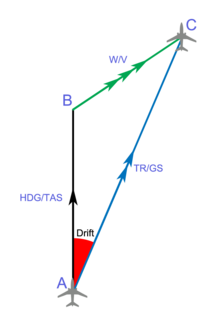
\includegraphics[width=0.4\textwidth]{Figures/dead_reck.png}
    \caption*{Fonte: Wikipedia.}
    \label{fig:Dead reckoning}
\end{figure}

Na navegação do \textit{Turtlesim}, o teorema de pitagoras é utilizado para calcular
a distância entre a mesma e o objetivo definido durante cada instante. Para isso foi utilizado a fórmula 
    $d = \sqrt{(x\textsubscript{f} - x\textsubscript{i})^2 + (y\textsubscript{f} - y\textsubscript{i})^2}$
. Nos quais x\textsubscript{f} e y\textsubscript{f} são as distâncias finais e x\textsubscript{i} e y\textsubscript{i} são as distâncias da tartaruga em determinado instante.

Assim, para calcular quanto que o \textit{Turtlesim} precisa girar faz o uso da trigonometria, para calcular o ângulo do qual a \textit{Turtlesim} está deslocada  em relação ao objetivo. Com isso, se faz o uso da fórmula de arctg na qual 
$\theta = \frac{y\textsubscript{f} - y\textsubscript{i}}{x\textsubscript{f} - x\textsubscript{i}} $
. Por fim, pegamos esse ângulo e subtraímos do ângulo atual da \textit{Turtlesim} para descobrir o quanto a tartaruga precisa rotacionar.

Para definir a velocidade da tartaruga multiplicamos a distância por uma constante e para descobrir o quanto ela precisa rotacionar multiplicamos a 
angulação por outra constante. Assim esses dados são publicados no topic
cmd\_vel para alterar a velocidade da turtle até que ela chegue no objetivo
especificado.

\section{Desafio Webots}

O Webots é uma plataforma opensource usada para simular robôs. 
Desse modo, o desafio consiste em utilizar essa plataforma para 
simular um robô chamado piooner3x, corrigindo o código já existente
e alterando ele para caso ele encontre uma luminária pare de se locomover.

A partir disso foram realizados os tutoriais dessa plataforma para 
ter conhecimento de como utilizá-la e como simular os robôs. 
Em seguida foi colocado um sensor de luz no piooner3x para que 
o mesmo tenha uma forma de detectar a luminosidade do ambiente
e seu código foi alterado para que se a leitura do sensor 
ultrapasse determinado valor ele pare.

\begin{figure}[h!]
    \centering
    \caption{Webots}
    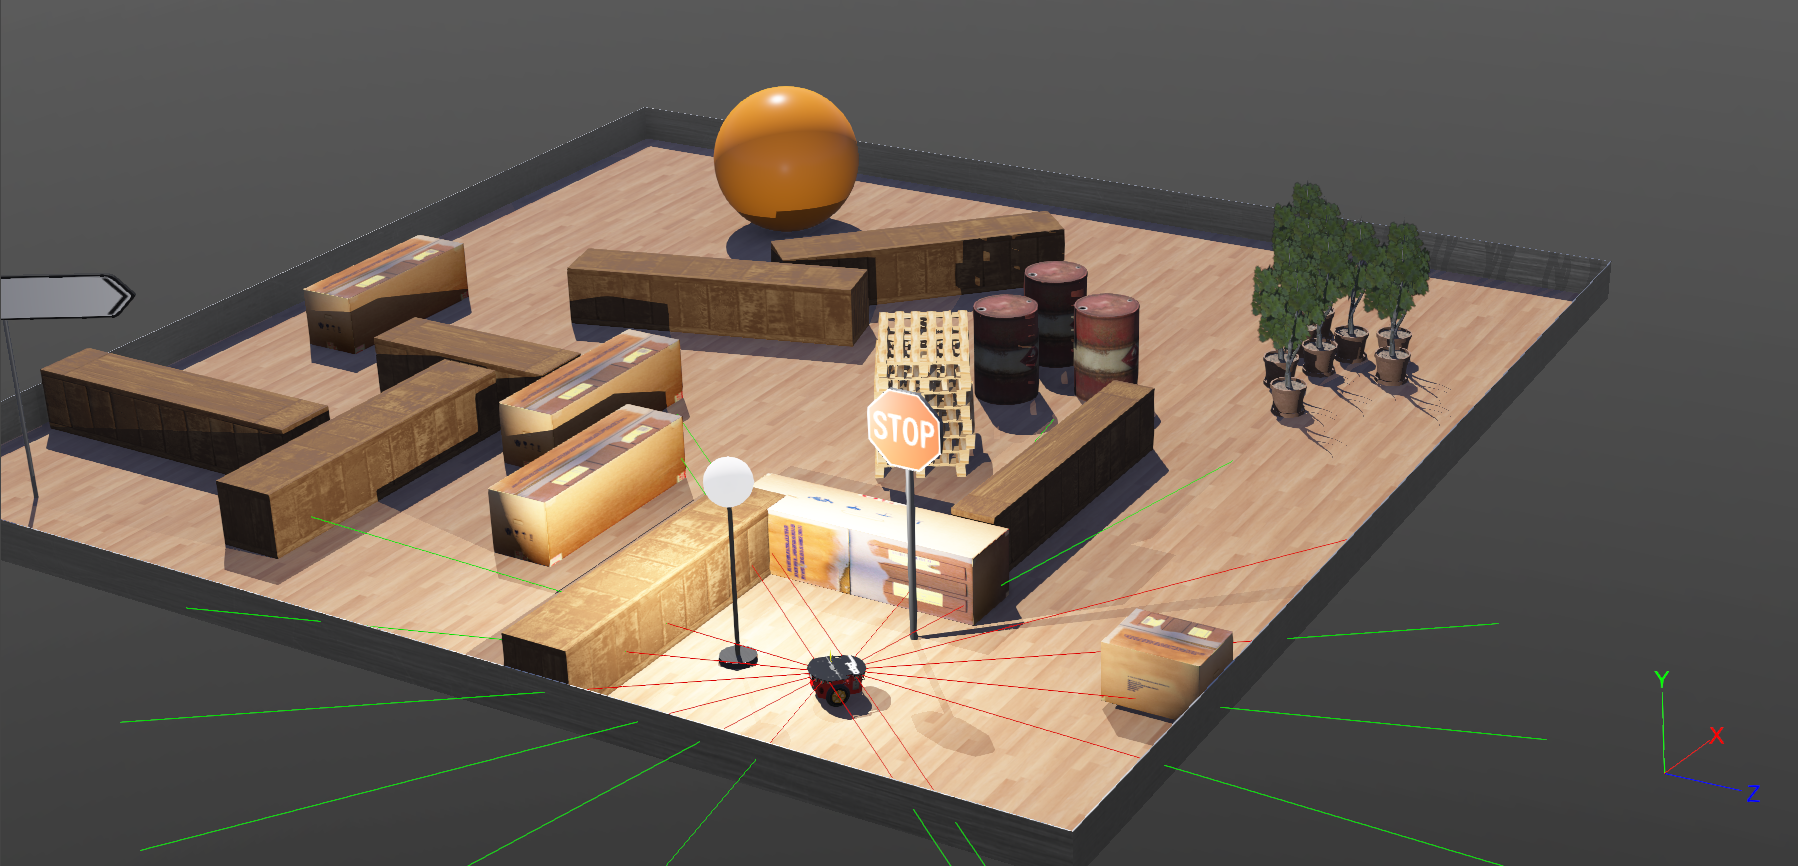
\includegraphics[width=1\textwidth]{Figures/webots3.png}
    \caption*{Fonte: Autoria propria.}
    \label{fig:Webots}
\end{figure}


\section{Desafio Husky}
Husky é um veículo UGV no qual atraves do ROS pode ser 
simulado em conjunto com o gazebosim e o rviz, sendo ambos
simuladores no qual o primeiro é voltado para o ambiente 
ao redor do husky e o segundo é como esse ugv percebe o mundo.
O desafio consiste em utilizar os simuladores para testar
diferentes formas de navegação com o husky.

O primeiro desafio é simular o husky com o package move base. 
Consiste em dar uma localização no mundo e ele irá tentar atingir 
esse objetivo. Caso o ugv identifique algum obstáculo ele irá desviar,
ou caso fique preso irá entrar em um processo chamado conservative reset
se parar de ficar preso voltará a navegação, caso não entrará em 
clearing rotation, se mesmo assim continuar preso iniciaram um aggressive reset
e continuando preso vai por fim fazer uma clearing rotation e se mesmo 
assim continuar preso vai abortar a ação. Como mostra na imagem \ref{fig:Move Base}.

%imagem https://wiki.ros.org/move_base

\begin{figure} [h!]
    \centering
    \caption{Move Base}
    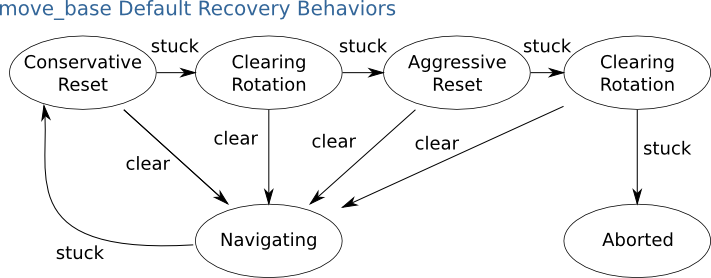
\includegraphics[width=0.8\textwidth]{Figures/recovery_behaviors.png}
    \caption*{Fonte: ROS Wiki.}
    \label{fig:Move Base}
\end{figure}

O segundo desafio é o amcl demo, o qual é a junção do move base com o
amcl. Assim o amcl é um sistema probabilístico de localização do robô
o qual através de sensores de laser fazem o tracking da posição do 
robô dentro de um mapa.


%imagem do simulador 

Gmapping demo é o terceiro desafio, ele é a junção do move base com o
gmapping. Esse package prove um SLAM (Simultaneous localization and mapping), 
baseado em sensores a laser. Com o gmapping é criado um mapa 2D do ambiente.
%Como pode ser mostrado na imagem abaixo.


%imagem do mapa

Por último foi realizado o frontier exploration demo, é composto 
pelo move base, gmapping, e o frontier exploration. Dessa forma,
o frontier em conjunto com esses packages para realizar a 
exploração de ambientes


